\section*{Br Konzentration}

Um die Br Konzentratio zu bestimmen werden die Daten aus der Absoprtionsmessung analysier.
Zunächst muss jedoch die Streuintensität abgezogen werden, dafür wird eine Baseline Intensität bestimmt.


Die Basline wir mithilfe von Matlab geffited um eine genauere Approximation zu erhalten.
Die Form der Baseline ist 
\begin{equation*}
    I_{\mathrm{Background}} = a \cdot x^4 + b
\end{equation*}

Angehangen sind die Ergebnisse des Fits, zur Datenermittlung wurde ein Edgefinder auf das Bild des Spektrums angewandt.
Die Daten wurden dann händisch aussortiert und nur die Schawarzen Datenpunkte zum fitten verwendet.

\begin{figure}[htbp]
    \centering
    
    \begin{subfigure}[b]{0.3\textwidth}
        \centering
        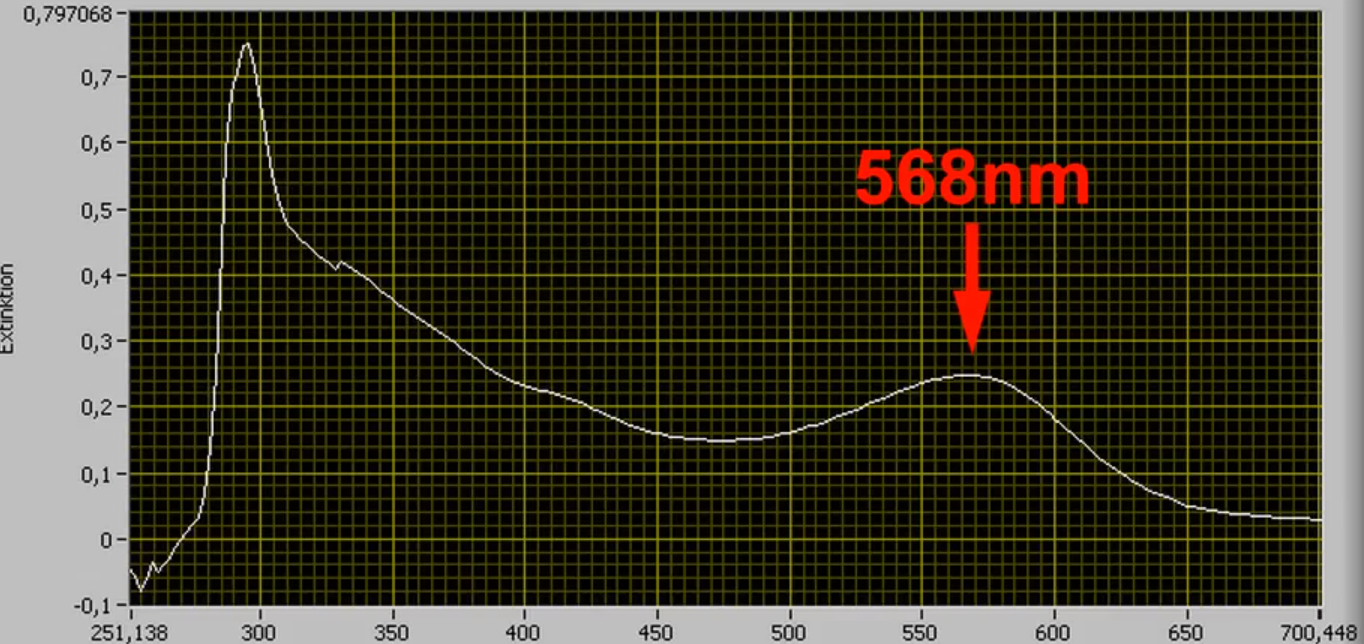
\includegraphics[width=\textwidth]{Spektrum.png}
        \caption{Spektrum der Absoprtionsmessung}
        \label{fig:Spektrum}
    \end{subfigure}
    \hfill
    \begin{subfigure}[b]{0.3\textwidth}
        \centering
        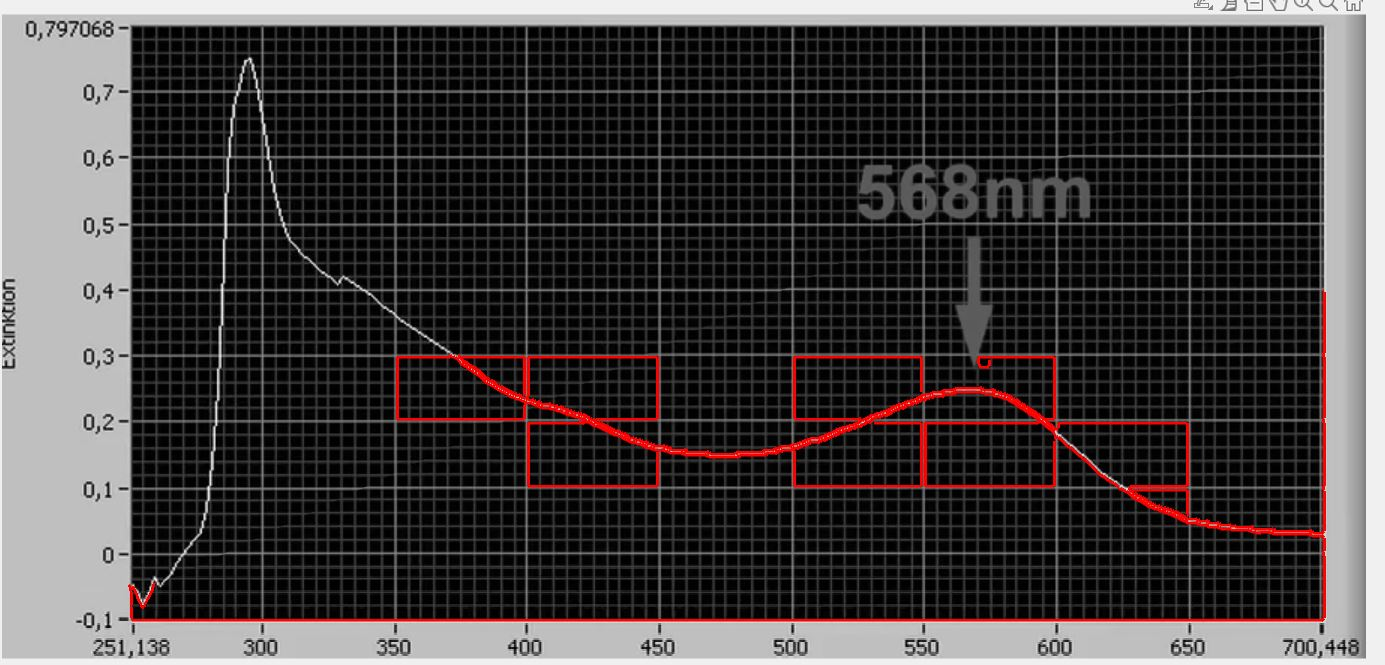
\includegraphics[width=\textwidth]{Data picture.JPG}
        \caption{Detektion der Daten}
        \label{fig:Datafind}
    \end{subfigure}
    \hfill
    \begin{subfigure}[b]{0.3\textwidth}
        \centering
        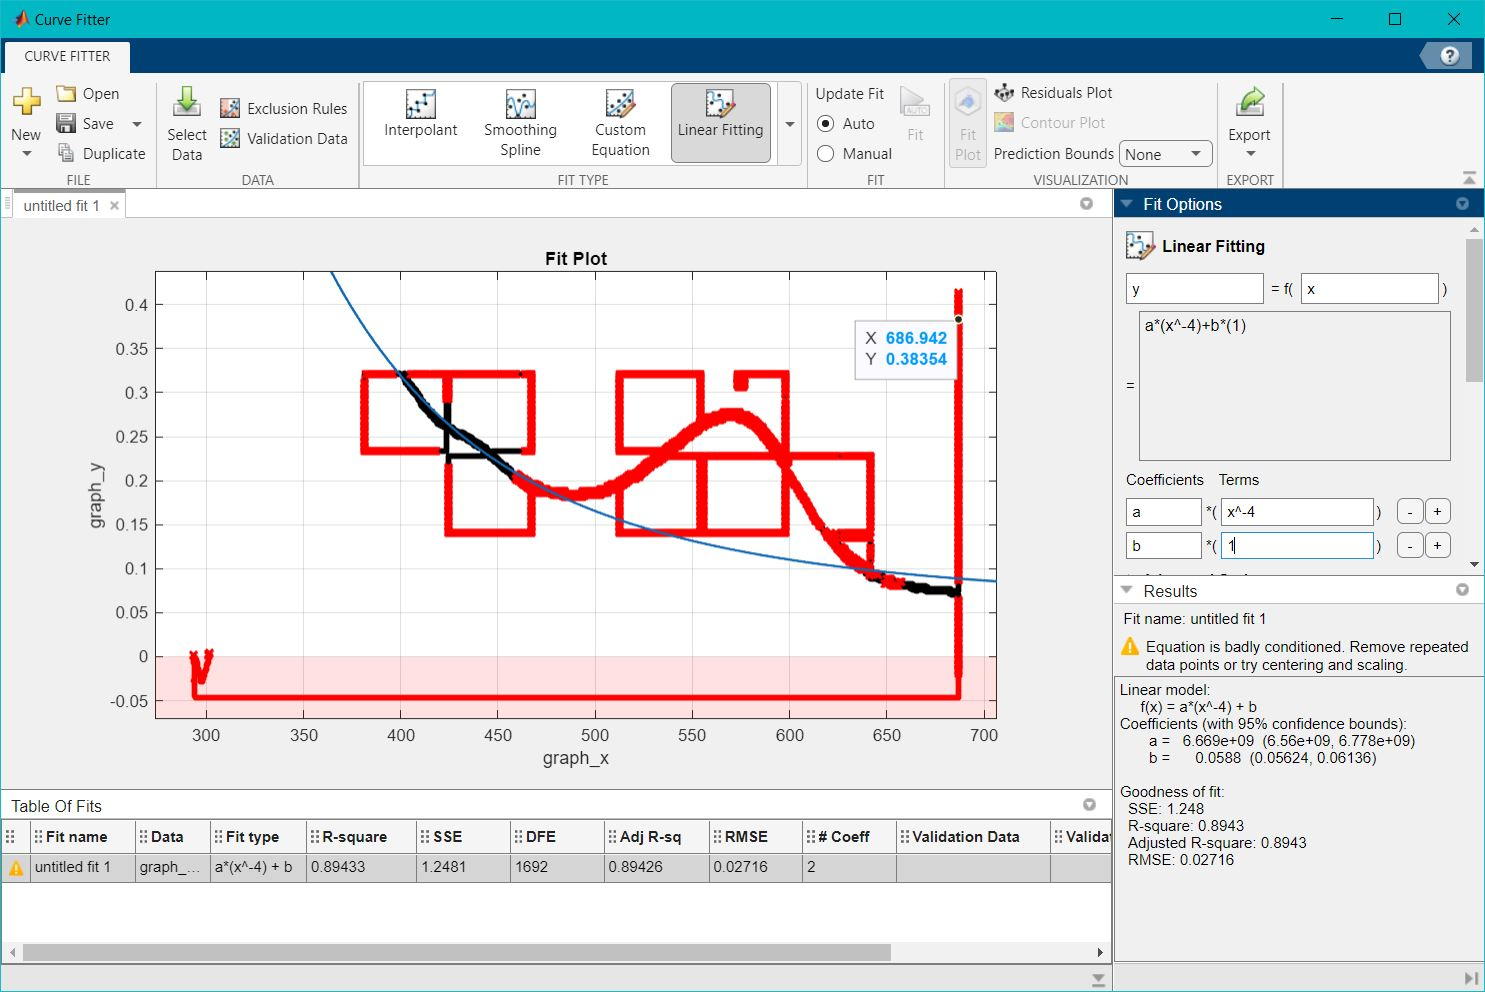
\includegraphics[width=\textwidth]{matlab fit.JPG}
        \caption{Fit des Hintergrunds}
        \label{fig:Fit}
    \end{subfigure}
    
    \caption{Prozess um Hintergrund zu bestimmen}
    \label{fig:Background}
\end{figure}

Der daraus ermittelte Wert für den Hintergrund ist
\begin{align*}
    y_{\mathrm{Background}} = 0,1229.
\end{align*}

Der Wert für die Extinktion ergibt sich aus der Differenz der Daten 
\begin{equation}
    E_{\mathrm{Peak}} = 0,2773 - 0,1229 = 0,1544
\end{equation}


